\documentclass[../main/thesis.tex]{subfiles}
\graphicspath{{/home/arefk/uio/MScThesis_AreKvanum2022_SeaIceML/thesis/performance_assessment/figures/}}
\begin{document}

\section{Comparing against physical models}
The purpose of this section is twofold. Firstly, it aims at describing the process of preparing samples from the Barents-2.5 and NeXtSIM forecasting systems which are comparable to the Machine Learning forecasts at lead times of one, two and three days. Secondly, the performance of the forecasting systems will be assessed against the Sea Ice Charts, which are assumed to be the ground truth.

\subsection{Short note on NIIEE}

\todo{Dette stemmer ikke lengre, enre i takt med at iskanten regnes ut for flere contours.}
Currently when computing the NIIEE, regardless of contour threshold, the same climatological ice edge length at concentration\_fraction = 15\% is used. The reasoning is twofold. First, the operational definition of the Marginal Ice Zone is sea ice within the concentration range $(15\% - 80\%)$ \citep{Dumont2022}, which allows the lower limit of the Marginal Ice Zone to serve as the value that define the Ice Edge. This definition is widely used in papers on verification metrics of the sea ice edge \citep{Dukhovskoy2015,Goessling2016,Goessling2018,Melsom2019}. Furthermore, the purpose of the climatological ice edge is to unify the different forecasts and benchmarks with a common sea ice edge length not biased towards any of the compared products. Hence, the same climatological sea ice edge at $sic = 15\%$ will be used as the normalization factor. However, it is noted that this approach should cause the higher concentration contours to have a smaller NIIEE than expected, as the higher concentration contours have a somewhat smaller area with a consequently shorter edge length. Though the difference should not be very large \missingfigure{Få inn figur som viser areal og ice edge length for alle concentartion ocntours for et forecast.}. Finally, since all forecasts are normalized using the same number, though their scale changes their size difference towards each other is intact.

\subsection{Preparing data}
The logic behind sample creation is similar for both physical models. The idea is that the bulletin date of the physical forecasting system is +1 the bulletin date of the machine learning forecast. Furthermore, a daily mean is computed from the forecast based on the lead time of the forecast. I.e., a 1 day lead time for the machine learning forecast would constitute a daily mean of the first 24 hours forecasted by a physical forecasting system starting at 00 the following day of the machine learning bulletin date. 

\begin{figure}
    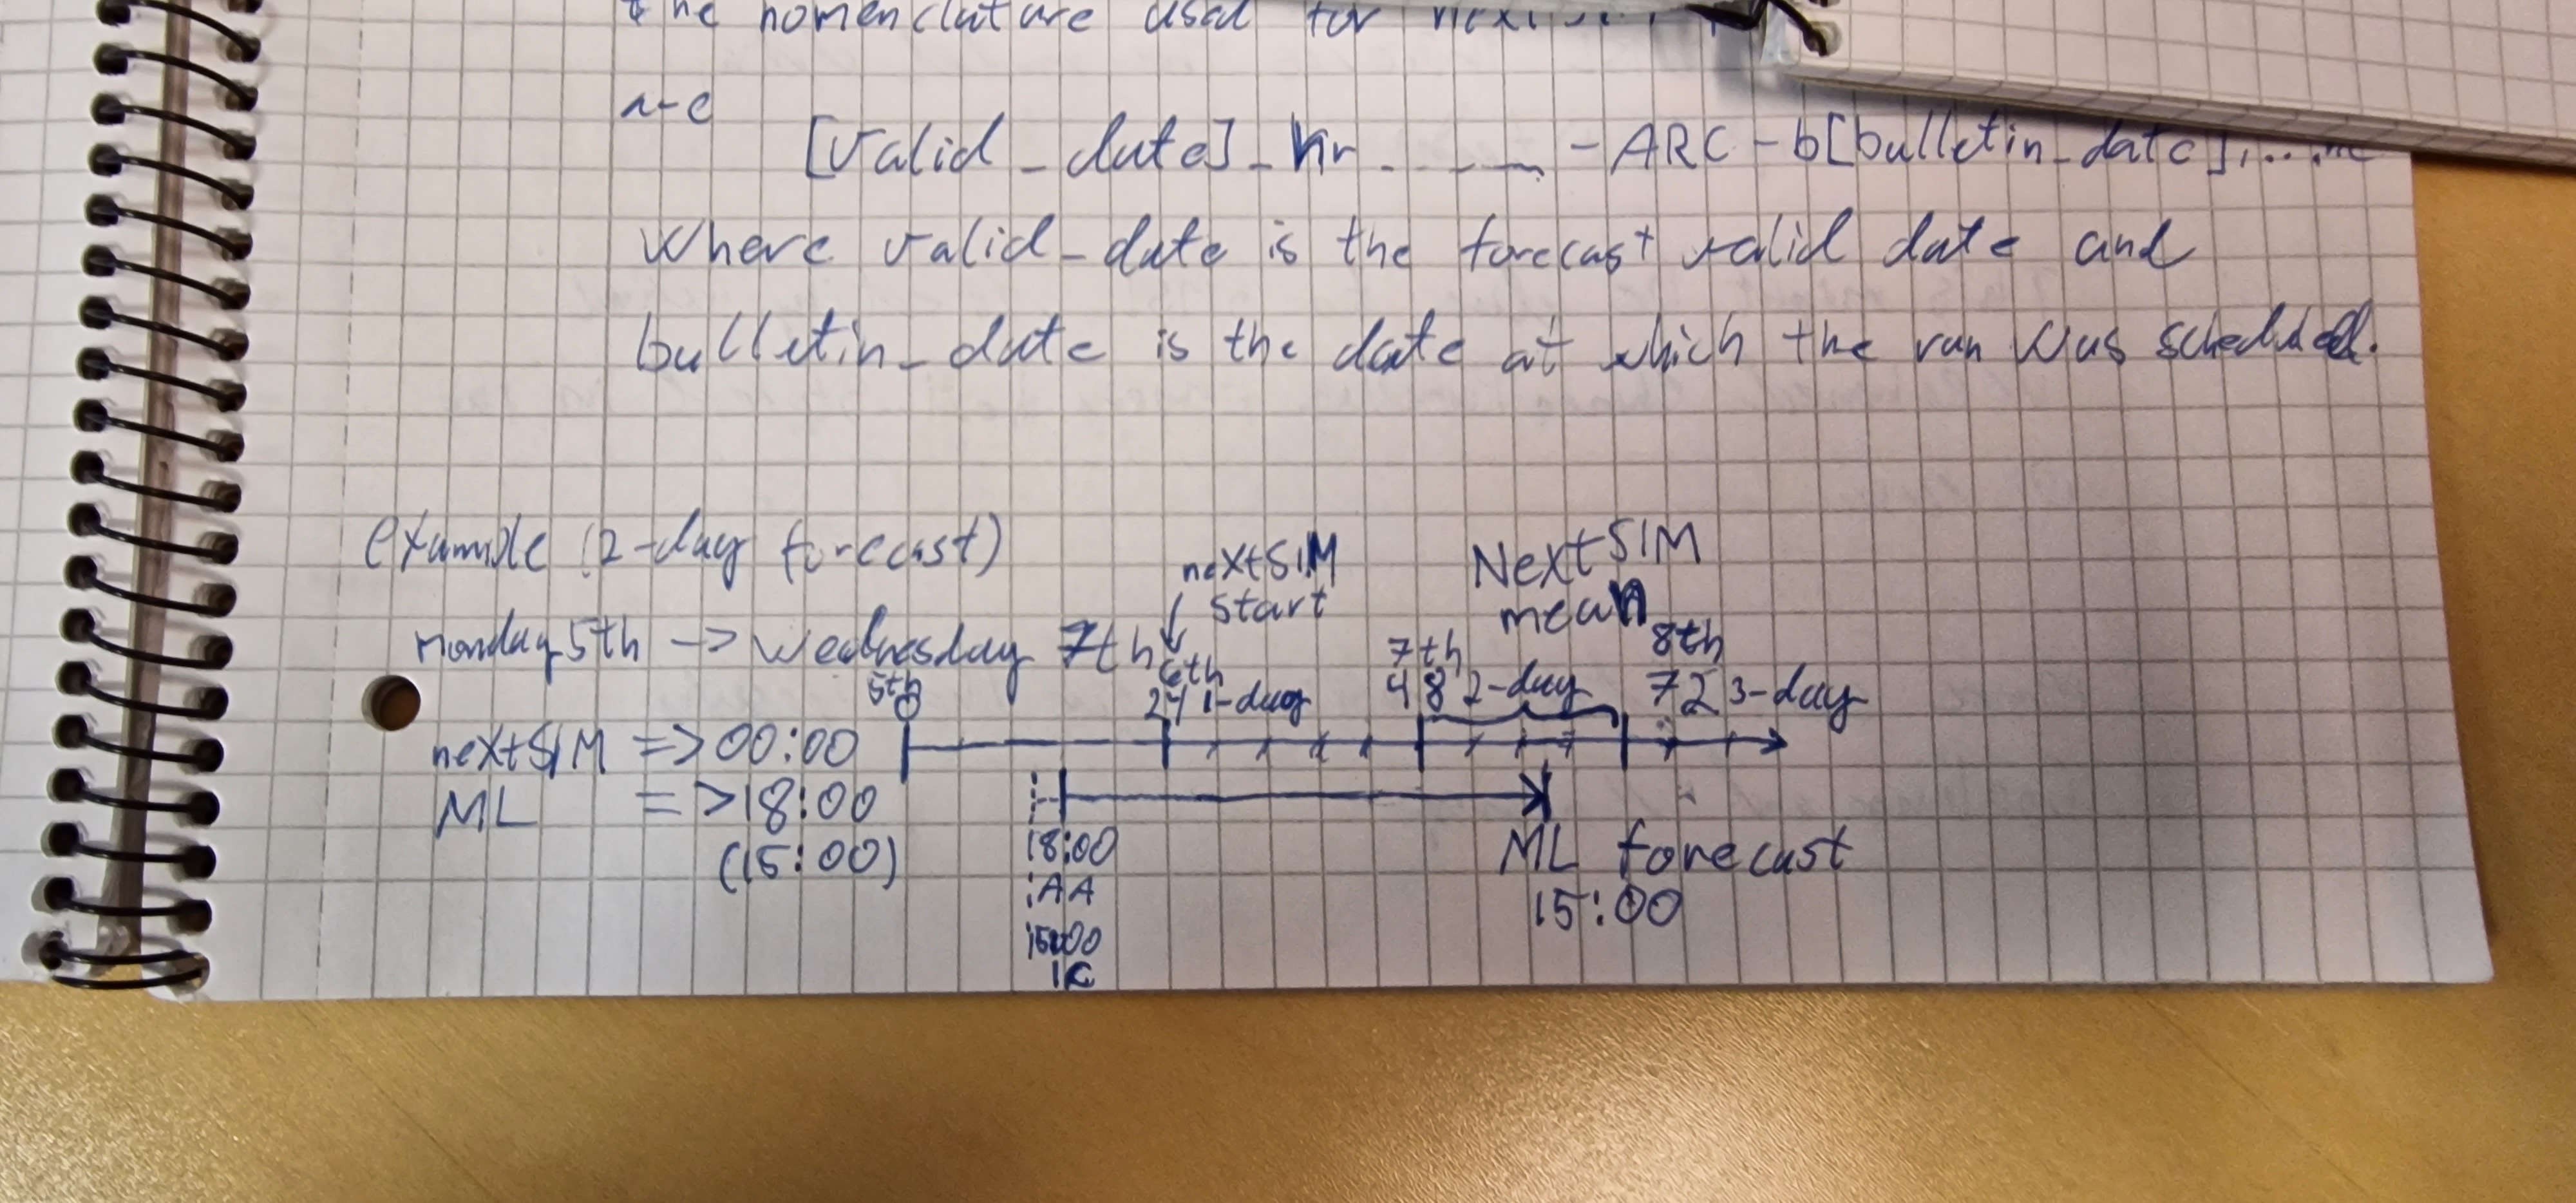
\includegraphics[width=0.93\textwidth]{forecast_sketch.jpg}
    \caption{\label{fig:physical_pipeline}Sketch presenting how physical model forecasts are compared against machine learning forecasts. The axis represents time after 00:00 bulletin date of the machine learning forecast. The machine learning forecast is initiated 6 hours prior to the start of the physical model. The sketch exemplifies how the 2-day lead time machine learning forecast at 15:00 (reality 45 hours) is compared against an entire second day of a physical forecast (lead times 24 - 47).}
\end{figure}
\todo{Figure (\ref{fig:physical_pipeline}) to be made professional, using e.g. TiX}


\biblio
\end{document}